
\chapter{基本事項}

\section{はじめに}

通常の変数と、確率変数を明確に区別して理解を進めていこう。
ここでいう「通常の」変数とは確率とは無関係に値を持つものであり、例えばその日の体重だったり身長だったり気温だったりするものである。
今日は60kgで、明日はX\%の確率で70kgになる、ということは無いため確率変数ではないと言える。
ただし、解釈によっては体重も確率変数になり得る。
日本人の平均体重を考えると、だいたい60~70kgが標準体重で、数\%の確率で100kgの人がいる、とか。

確率変数は$X$で表され、通常の変数は$x$で表される。

\section{基礎知識}

\subsubsection{平均 $\bar{x}$}

実験の$n$個の測定値($x_1,x_2,...,x_n$)の代表値として、平均は(mean;算術平均または相加平均)がよく用いられる:
\begin{equation}
  \bar{x} = \frac{x_1 + x_2 + ... + x_n}{n}  = \frac{1}{n} \sum_{i=1}^{n} x_i
\end{equation}


\subsubsection{分散 $V$}

各測定値が、平均からどれくらい離れて分布しているか(どれだけばらついているか)を表す指標として分散が用いられる。
分散は平均からのズレ(偏差)の二乗和の平均であり、次のように定義される:
\begin{equation}
  V= \sigma^2 = \frac{1}{n}\sum_{i=1}^{n} (x_{i}-\bar{x})^{2} = \int (x-\bar{x})^2f(x)dx
\end{equation}
平均値の周りにピッタリ分布していれば、 分散は小さくなり、平均値よりも大きかったり小さかったりすると、分散$V$は大きくなる。
また分散の平方根を取ったものを標準偏差$S$という。

\subsubsection{期待値}
ある確率変数$x$に対する期待値は$E[x]$と表され、
\begin{equation}
  E[x] = \sum_{i=1}^{n} x_i p_i 
\end{equation}
と表される。ここで$p_i$は$x_i$を観測する確率である\footnote{サイコロを投げる例であれば、1回投げて$x=$1の目が出る確率は$p=$1/6。}。
$x$が全て等確率で出現するのであれば(ex.理想的なサイコロの例)、
\begin{equation}
  E[x] = \frac{1}{n}\sum_{i=1}^{n} x_i
\end{equation}
と表される。
連続な値を取る確率密度関数に従う場合であれば$x$を観測する確率は$f(x)$と表されるので、
\begin{equation}
  E[x] \coloneqq \int xf(x)dx
  \label{eq:fundamental_concepts:expectation_value}
\end{equation}
と積分形式で表すことができる。

\begin{itembox}[l]{Gaussianの期待値}
  ガウス分布に従う変数の期待値を計算すると:
  \begin{equation}
    E[x] = \int_{-\infty}^{\infty} x \frac{1}{\sqrt{2\pi\sigma}} \exp^{-\frac{(x-\mu)^2}{2\sigma^2} } dx
  \end{equation}
\end{itembox}


確率によって重み付けして平均を計算したもので、
\begin{equation}
  E[x] = \frac{p_1\times x_1+ p_2\times x_2+...+ p_n \times x_n}{n} = \frac{1}{n}\sum_{i=1}^{n} p_ix_i
\end{equation}
重要な性質として、実験結果$x=(x_1,x_2,...,x_n)$の期待値は、
\begin{equation}
  E[x] = \lim_{n\to\infty} = \frac{1}{n}\sum_{i=1}^{n} p_ix_i = \frac{1}{n}\sum_{i=1}^{n} p_ix_i
\end{equation}



\subsubsection{母集団と標本}
ある母集団から確率変数$X$を予想する場合。無限個のサンプル取得が可能であれば、 $X$の平均値(=期待値)は

\begin{equation}
  \mu = \bar{X} = \lim_{n\to\infty} \left(\frac{1}{n} \sum_{i=1}^{n} x_i \right)
\end{equation}

母平均の期待値 $E[\mu]$は、
\begin{equation}
  E[\mu] = \lim_{n\to\infty}\sum_{i=1}^{n}
\end{equation}

で表される。母集団から無限個のサンプルを取得すれば、真の値(母平均)を計算することができることを意味する。
また、母集団の分散(母分散)は

\begin{equation}
  V= \frac{1}{n}\sum_{i=1}^{n} (x_{i}-\mu)^{2}
\end{equation}

で表される。

実際には$n$の値は有限であり、母平均$\mu$や母分散$V$を計算することはできない。
ここで注意が必要である。
\subsubsection{標本分散}
\begin{equation}
  E((X-\bar{X})^2) = \sum_{i=1}^{n} (X_i - \bar{X})^2 = \sum_{i=1}^{n} \left(X_i - \frac{1}{n}\sum_{j=1}^{n} X_j \right)^2
  =
\end{equation}

% ====================================
\section{確率分布}
\subsubsection{ポワソン分布}
\label{subsubsec:poisson}
平均 $\lambda$ 回発生する確率事象が、$x$ 回起こる確率

\begin{table}[h]
  \centering
  \begin{tabular}{lll}
    確率密度関数 & $f(x)=\frac{e^{\lambda}~\lambda^{x}}{x!}$   \\
    期待値      & $E(x)=\lambda$    \\
    分散        & $V(x)=\lambda$
  \end{tabular}
\end{table}

事象が起こる平均値$\lambda$が大きくなるほど、形がガウス分布に近づいていく。
十分に大きくなると$\mu=\lambda$、$V=\lambda$のガウス分布として近似できる。

\begin{figure}[h]
  \centering
  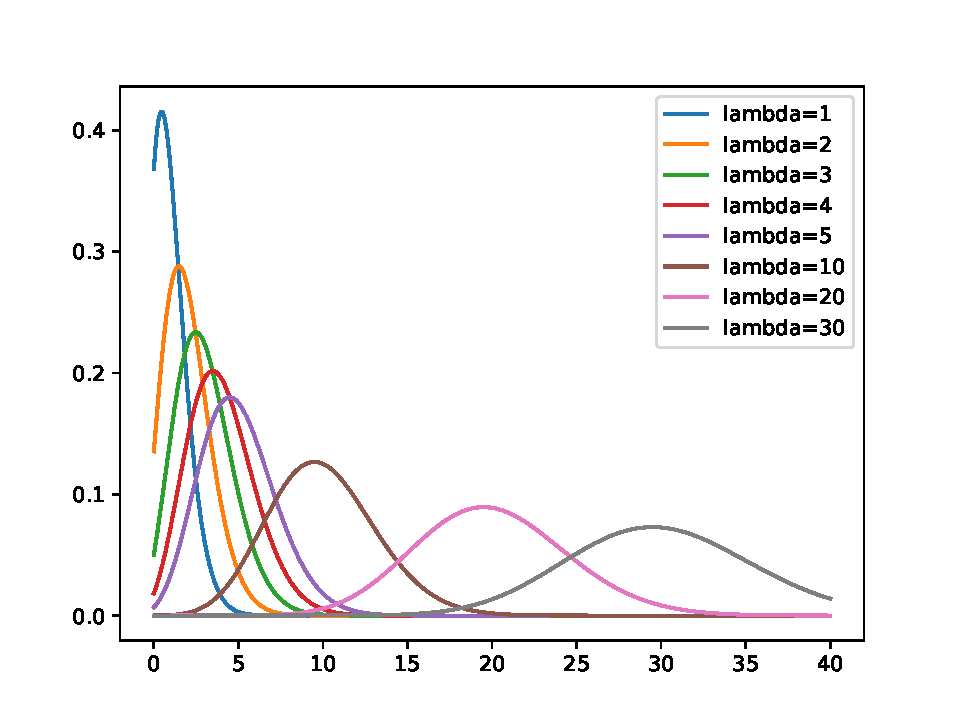
\includegraphics[scale=0.5]{python/poisson_scan.pdf}
  \caption{異なる平均値を取ったときのポワソン分布。平均$\lambda$が大きくなるほど、ガウス分布のような形状になっていくのが分かる。}
\end{figure}

\subsubsection{正規分布(ガウス分布)}

\begin{table}[h]
  \centering
  \begin{tabular}{lll}
    確率密度関数 & $f(x)=\frac{1}{\sqrt{2\pi} \sigma}e^{-\left(\frac{(x-\mu)^2}{2\sigma^2}\right)}$   \\
    期待値      & $E(x)=\mu$    \\
    分散        & $V(x)=\sigma$
  \end{tabular}
\end{table}

\begin{itembox}[l]{ガウス分布の性質その1}
  確率変数$X$が$N(\mu,\sigma^2)$の正規分布に従うなら、$aX+b$は$N(a\mu+b,a^2\sigma^2)$の正規分布に従う
\end{itembox}





% ===================================================== %
\section{共分散}
% ===================================================== %

\subsection{モーメント}
確率密度関数$f(x)$に対して、$x^n$の期待値を定義することができる($n$は整数)。
それらはモーメントと呼ばれ:
\begin{equation}
  a_n \coloneqq E[x^n]
\end{equation}
と定義される。\refeq{eq:fundamental_concepts:expectation_value}より
\begin{equation}
  a_n = \int x^n f(x) dx
\end{equation}
と表される。$n=1$の場合は平均値を表す。

また、$x$が平均値からどれだけ離れているか(散らばっているか)を表す量として中央モーメント
\begin{equation}
  m_n \coloneqq E[(x-\mu)^n]
\end{equation}
が定義されている。
$n=2$は分散として知られている値であり、
\begin{equation}
  m_2 = E[(x-\mu)^2] = \sigma^2 = V[x]
\end{equation}


\subsection{共分散の定義}

確率密度関数が2変数に依存する場合($f(x,y)$)、共分散(covariance)として変数同士の関係性を計算することができる:
\begin{equation}
  \begin{split}
    \mathrm{cov}[x,y]
    & \coloneqq \frac{1}{n} \sum_{i=1}^{n} (x_i-\bar{x})(y_i - \bar{y})  \\
    & = \frac{1}{n} \sum (x_iy_i - x_i\bar{y} - \bar{x}y_i + \bar{x}\bar{y})) \\
    & = \frac{1}{n} \sum x_iy_i - \frac{1}{n}\bar{y} \sum x_i - \frac{1}{n} \bar{x}\sum  y_i + \bar{x}\bar{y} \\
    & = \frac{1}{n} \sum x_iy_i - \frac{1}{n}\bar{y} \sum x_i \\
    & = E[xy] - E[x]E[y]
  \end{split}
\end{equation}
また連続関数を用いると
\begin{equation}
  \mathrm{cov}[x,y] = \int xyf(x,y) dxdy - \int xf(x,y)dx \int yf(x,y)dy
\end{equation}
$f(x,y)=f(x) \cdot f(y)$と表すことができるなら(互いに独立な事象の場合)、
\begin{equation}
  \mathrm{cov}[x,y] = E[xy] - E[x]E[y] = \iint xyf(x)f(y) dxdy - \int xf(x) dx - \int yf(y) dy = 0
\end{equation}
となる。
\ref{fig:fundamental_concepts:covariance}に共分散によるデータの分布の違いを示している。
\begin{figure}
  \centering
  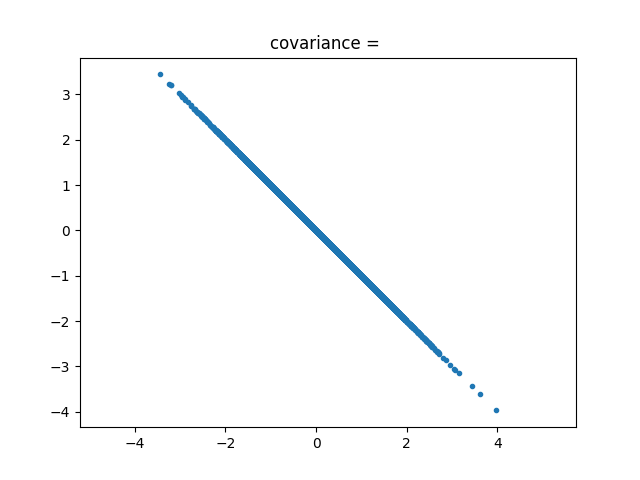
\includegraphics[width=0.3\textwidth]{figure/fundamental_concepts/covariance_-1}
  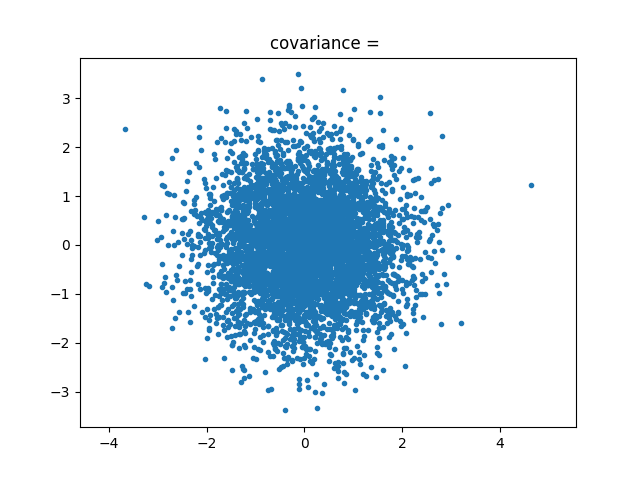
\includegraphics[width=0.3\textwidth]{figure/fundamental_concepts/covariance_0}
  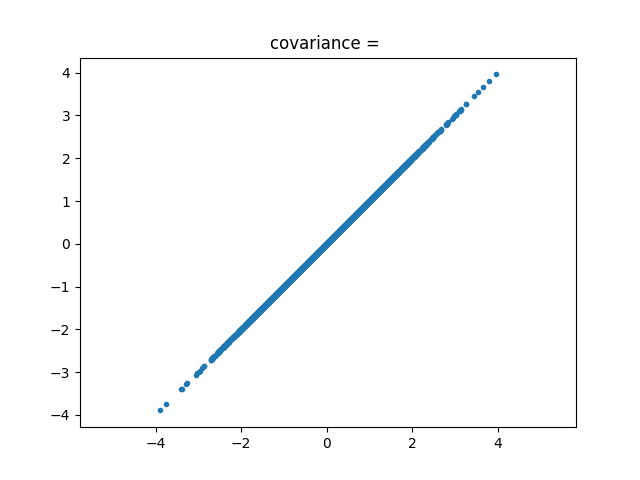
\includegraphics[width=0.3\textwidth]{figure/fundamental_concepts/covariance_1}
  \caption{
    左から順に、cov=-1, 0, +1 の共分散の関係性を持たせてプロットした図。
  }
  \label{fig:fundamental_concepts:covariance}
\end{figure}

また、相関(correlation)として次の量も定義される:
\begin{equation}
  \rho \coloneqq \frac{\mathrm{cov}[x,y]}{\sigma_x\sigma_y}
\end{equation}

これらは多次元への拡張も可能である。
\begin{eqnarray}
  V_{i,j}   &=& \mathrm{cov}[x_i, x_j] = E[x_i x_j] - E[x_i]E[x_j], \\
  \rho_{i,j}&=& \frac{V_{ij}}{\sigma_{i}\sigma_{j}}
\end{eqnarray}


\subsection{共分散行列}


\subsection{多変量正規分布}

Multivariate nominal distribution(多変量正規分布)は:
\begin{equation}
  f(\bm{x}|\mu, \Sigma) = \frac{1}{\sqrt{(2\pi)^N |\Sigma|}} \exp \left( -\frac{1}{2}(\bm{x}-\mu)^T \Sigma^{-1} (\bm{x}-\mu) \right) \coloneqq \mathcal{N}(\mu,\Sigma)
\end{equation}
と定義される。$\bm{x}$は多次元の変数、$\mu$は平均値ベクトル、$\Sigma$は$N\times N$共分散行列、$|\Sigma|$は行列式を表す。



